	\subsection{UC1 - Web App - Autenticazione}
		
		\begin{figure}[t!]
			\centering
			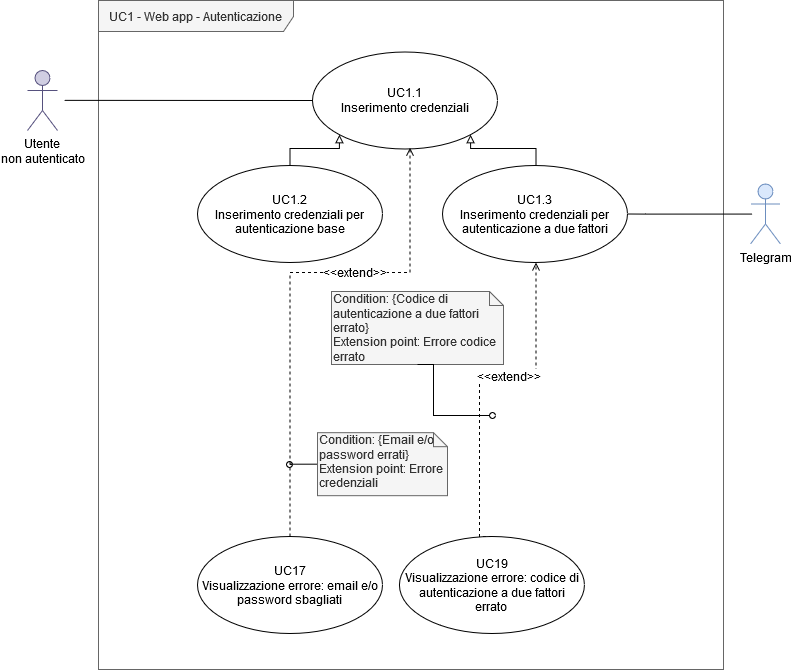
\includegraphics[height=10em]{res/images/uc1}
		\end{figure}
		

		\subsubsection{UC 1.1 - Visualizzazione form di autenticazione}

		\begin{itemize}
			\item \textbf{Attori Primari}: utente non autenticato.
			\item \textbf{Descrizione}: L'utente tenta di autenticarsi nella web-application mediante un form che richiede la compilazione obbligatoria di alcuni campi.
			\item \textbf{Precondizione}: L'utente visualizza la schermata di login con il relativo form.
			\item \textbf{Postcondizione}: L'utente effettua la login e in base alle credenziali inserite viene identificato come un altro attore (Utente autenticato, Moderatore ente o Amministratore) con i relativi privilegi.
			\item \textbf{Scenario Principale}:
			\begin{enumerate}
				\item L'utente compila i campi del form;
				\item L'utente preme il pulsante di login.
			\end{enumerate}
			\item \textbf{Inclusioni}:
				\begin{itemize}
					\item Compilazione email e password (UC 1.2).
				\end{itemize}
			\item \textbf{Estensioni}:
				\begin{itemize}
					\item Errore: viene inserita una email o una password sbagliata (UC 1.4);
					\item Errore: L'utente non ha i permessi necessari per accedere (UC 1.5).
				\end{itemize}
		\end{itemize}

		\subsubsection{UC 1.2 - Compilazione email e password}
		\begin{itemize}
			\item \textbf{Attori Primari}: utente non autenticato.
			\item \textbf{Descrizione}: L'utente compila i campi del form: email e password.
			\item \textbf{Precondizione}: L'utente visualizza la schermata di login con il relativo form.
			\item \textbf{Postcondizione}: L'utente ha compilato i campi email e password.
			\item \textbf{Scenario Principale}:
			\begin{enumerate}
				\item L'utente compila il campo con la email;
				\item L'utente compila il campo con la password.
			\end{enumerate}	
			\item \textbf{Estensioni}:
			\begin{itemize}
				\item Viene richiesta l'autenticazione a due fattori per proseguire (UC 1.3);
				\item Errore: il codice per l'autenticazione a due fattori è errato (UC 1.6).
			\end{itemize}
		\end{itemize}

		\subsubsection{UC 1.3 - Richiesta autenticazione a due fattori}
		\begin{itemize}
			\item \textbf{Attori Primari}: utente non autenticato;
			\item \textbf{Attori Secondari}: \glock{Telegram};
			\item \textbf{Descrizione}: L'utente, a seguito della verifica delle proprie credenziali e sulla base delle proprie impostazioni, deve eventualmente inserire un codice per l'autenticazione a due fattori.
			\item \textbf{Precondizione}: L'utente ha inserito delle credenziali che sono risultate corrette e gli viene richiesto di inserire un codice.
			\item \textbf{Postcondizione}: L'utente ha inserito il codice per l'autenticazione.
			\item \textbf{Scenario Principale}:
			\begin{enumerate}
				\item \glock{Telegram} emette una notifica all'utente indicando il codice di autenticazione;
				\item L'utente riceve tramite \glock{Telegram} il codice di autenticazione;
				\item L'utente inserisce il codice di autenticazione.
			\end{enumerate}	
		\end{itemize}

		\subsubsection{UC 1.4 - Errore email o password}
		\begin{itemize}
			\item \textbf{Attori Primari}: utente non autenticato;
			\item \textbf{Descrizione}: L'utente prova ad autenticarsi ma inserisce una email o una password che non coincidono con quelle salvate nel database, quindi visualizza un errore.
			\item \textbf{Precondizione}: L'utente ha sbagliato ad inserire la email o la password.
			\item \textbf{Postcondizione}: Viene visualizzato un errore relativo alla email o la password.
			\item \textbf{Scenario Principale}:
			\begin{enumerate}
				\item L'utente prova ad accedere usando una email o una password errati.
			\end{enumerate}	
		\end{itemize}

		\subsubsection{UC 1.5 - Errore utente non autorizzato}
		\begin{itemize}
			\item \textbf{Attori Primari}: utente non autenticato;
			\item \textbf{Descrizione}: L'utente prova ad autenticarsi ma non ha i privilegi per visualizzare nulla, quindi visualizza un errore.
			\item \textbf{Precondizione}: L'utente prova ad accedere non avendo i permessi necessari.
			\item \textbf{Postcondizione}: L'utente visualizza un errore riguardo la mancanza di permessi.
			\item \textbf{Scenario Principale}:
			\begin{enumerate}
				\item L'utente riceve un messaggio di errore indicante la mancanza di permessi.
			\end{enumerate}	
		\end{itemize}

		\subsubsection{UC 1.6 - Errore codice autenticazione a due fattori}
		\begin{itemize}
			\item \textbf{Attori Primari}: utente non autenticato;
			\item \textbf{Descrizione}: L'utente prova ad autenticarsi ma ha inserito un codice errato, quindi visualizza un errore.
			\item \textbf{Precondizione}: L'utente prova ad accedere inserendo un codice errato.
			\item \textbf{Postcondizione}: L'utente visualizza un errore riguardo il codice errato.
			\item \textbf{Scenario Principale}:
			\begin{enumerate}
				\item L'utente riceve un messaggio di errore che segnala che il codice di autenticazione è errato.
			\end{enumerate}	
		\end{itemize}